% +--------------------------------------------------------------------+
% | LaTeX Template                                                     |
% | for K-State Electronic Theses, Dissertations, and Reports          |
% |                                                                    |
% | Comments and guidelines for using the template are shown           |
% | within boxes like this one.                                        |
% |                                                                    |
% | Revised 6/30/06                                                    |
% | 9/14/06: Removed typos                                             |
% | 3/29/13: Commented out hypernat package                            |
% | 4/5/13: Changed to plain bib style
% | 5/17/13: added /cleardoublepage and /phantomsection to
% |          /bibliography to correct TOC page problem
% | 5/17/13: Fixed TOC problem with Dedication, Preface, etc.          |
% +--------------------------------------------------------------------+

% +--------------------------------------------------------------------+
% | Your paper should contain the following sections, except where     |
% | indicated as optional, in the order shown.  Also, all headings     |
% | shown with an asterisk (*) must be centered and in uppercase       |
% | letters:                                                           |
% |                                                                    |
% | Abstract Title Page (doctoral dissertations only)                  |
% | ABSTRACT* (doctoral dissertations only)                            |
% | Title Page                                                         |
% | Copyright Page (Optional - only needed if copyrighting)            |
% | ABSTRACT *                                                         |
% | TABLE OF CONTENTS *                                                |
% | LIST OF FIGURES *                                                  |
% | LIST OF TABLES*                                                    |
% | ACKNOWLEDGMENTS* (Optional)                                        |
% | DEDICATION * (Optional)                                            |
% | PREFACE * (Optional)                                               |
% | Individual Chapters                                                |
% | References and/or bibliography                                     |
% | Appendices (as needed)                                             |
% +--------------------------------------------------------------------+

% +--------------------------------------------------------------------+
% | The LaTex keyword \documentclass selects a particular class to     |
% | associate with the document.  The current documentclass            |
% | {class_diss} generates a Table of Contents that has leading dots   |
% | only on chapter subheadings.  If you prefer a Table of Contents    |
% | that has leading dots for all entries, replace {class_diss}        |
% | with {Mydiss} in the command below.                                |
% |                                                                    |
% +--------------------------------------------------------------------+

\documentclass[final, 12pt,oneside]{class_diss}

% +--------------------------------------------------------------------+
% | The bibliography style is set to a generic superscript. Other      |
% | styles are available in the styles directory.  To use an           |
% | author/year style, you'll need to make several adjustments:        |
% |   1.  In the \bibliographystyle command below, replace "unsrtnat"  |
% |       with the desired style from the \styles directory, e.g.,     |
% |       \bibliographystyle{styles\apa}                               |
% |   2.  In the \bibpunct command (several lines below), change the   |
% |       "s" to an "a"                                                |
% |   3.  Use "\citep" rather than "\cite" when making a citation in   |
% |       the text.                                                    |
% +--------------------------------------------------------------------+

\bibliographystyle{alpha}

% +--------------------------------------------------------------------+
% | Now, we add in all external packages that we will use throughout   |
% | the document.  You can add other packages as needed.
% +--------------------------------------------------------------------+

%\usepackage{     caption2} % Customize captions a bit more
\usepackage{      amsmath} % American Mathematics Society standards
%\usepackage{      wrapfig} % Wraps text around a figure or table
\usepackage{     graphicx} % Extended graphics package.
%\usepackage{     fancyhdr} % Efficiently handles headers and footers
%\usepackage{       braket} % Bra-Ket notation package
%\usepackage{     mathrsfs} % Specialized Math fonts (Hamiltonian, etc.)
%\usepackage{boxedminipage} % Boxed text can be produced
%\usepackage{     setspace} % Controls line spacing via \begin{space}

\usepackage{amsxtra}
\usepackage{amssymb}
\usepackage{amsthm}
\usepackage{latexsym}
\usepackage{setspace}
\usepackage[T1]{fontenc}    % Added by Jakub Jedryszek to support < and > in text
\usepackage[utf8]{inputenc} % Added by Jakub Jedryszek to support non-English letters
\usepackage{longtable}      % Added by Jakub Jedryszek to support tables bigger than 1 page


% +--------------------------------------------------------------------+
% | The color package allows one to select colors for hyperlinking     |
% | (see below).                                                       |
% +--------------------------------------------------------------------+

\usepackage[usenames]{color}

% +--------------------------------------------------------------------+
% | Colors defined for use with this template.                         |
% +--------------------------------------------------------------------+

\definecolor{Pink}{rgb}{1.0, 0.5, 0.5}
\definecolor{Maroon}{rgb}{0.8, 0.0, 0.0}

% +--------------------------------------------------------------------+
% | Added by Jakub Jedryszek for code snippets                         |
% | http://en.wikibooks.org/wiki/LaTeX/Source_Code_Listings            |
% +--------------------------------------------------------------------+

\usepackage{listings}

\definecolor{mygreen}{rgb}{0,0.6,0}
\definecolor{mygray}{rgb}{0.5,0.5,0.5}
\definecolor{red}{rgb}{0.6,0,0}
\definecolor{mymauve}{rgb}{0.58,0,0.82}

% Support syntax highlighting for AADL

\lstdefinelanguage{aadl}
{
    morekeywords = {in,out,package,end,bus,data,thread,port,group,process,processor,
        system,memory,device,subprogram,public,private,event,property,set,applies,to,
        units,type,implementation,parameter,reference},
    morekeywords = {properties,features,annex,modes,connections,flows,
        subcomponents,calls,binding},
    morekeywords = {aadlinteger,aadlboolean,aadlstring,aadlfloat},
    morecomment = [l]{--},
}

\lstdefinelanguage{bless}
{
    morekeywords = {all,skip,fetchadd,computation,availability,spread,swap,real,do,numberof,D,stop,invariant,not,integer,now,string,mod,d,iff,timeout,exists,implies,are,transitions,xor,for,fetchxor,sum,state,rational,rem,shared,C,bold,variant,post,throw,c,cor,of,nonvolatile,forall,or,pre,variables,bound,boolean,false,array,initial,.,type,final,on dispatch,B,complete,that,assert,catch,e,true,count,b,f,until,record,while,declare,def,and,cand,constant,states,in,null,setmode,if,fetchor,in mode,F,when,enumeration,complex,units,A,product,E,tops,fi,a,natural,modes,fetchand,fresh},
    morecomment = [l]{--},
}

\lstdefinelanguage{ada2012}
{
    morekeywords = {abort, else, new, return, abs, elsif, not, reverse, abstract, end, null, accept, entry, select, access, exception, of, separate, aliased, exit, or, some, all, others, subtype, and, for, out, synchronized, array, function,     overriding, at, tagged, generic, package, task, begin, goto, pragma, terminate, body, private, then, if, procedure, type, case, in, protected, constant, interface, until, is, raise, use, declare, range, delay, limited, record, when, delta, loop, rem, while, digits, renames, with, do, mod, requeue, xor},
    morecomment = [l]{--},   
}

% Layout for listings

%\lstset{language=aadl,
%        basicstyle=\scriptsize\sffamily,
%        aboveskip=.1cm, % \smallskipamount, % \bigskipamount,
%        belowskip= \smallskipamount, % \bigskipamount,
%        abovecaptionskip=-.5cm, % \smallskipamount, % \medskipamount,
%        belowcaptionskip=.0cm, % \smallskipamount, % \bigskipamount,
%        xleftmargin=.0cm,
%        captionpos=b,
%        tabsize=3,
%        }

\lstset{ %
  backgroundcolor=\color{white},   % choose the background color; you must add \usepackage{color} or \usepackage{xcolor}
  basicstyle=\footnotesize\ttfamily,        % the size of the fonts that are used for the code
  breakatwhitespace=false,         % sets if automatic breaks should only happen at whitespace
  breaklines=true,                 % sets automatic line breaking
  captionpos=b,                    % sets the caption-position to bottom
  columns=fullflexible,
  commentstyle=\color{mygreen},    % comment style
  %deletekeywords={...},            % if you want to delete keywords from the given language
  escapeinside={\%*}{*)},          % if you want to add LaTeX within your code
  extendedchars=true,              % lets you use non-ASCII characters; for 8-bits encodings only, does not work with UTF-8
  %frame=single,                    % adds a frame around the code
  keepspaces=true,                 % keeps spaces in text, useful for keeping indentation of code (possibly needs columns=flexible)
  keywordstyle=\bf,       % keyword style
  language=Ada,                    % the language of the code
  %morekeywords={*,...},            % if you want to add more keywords to the set
  numbers=none,                    % where to put the line-numbers; possible values are (none, left, right)
  numbersep=2,                   % how far the line-numbers are from the code
  numberstyle=\tiny\color{mygray}, % the style that is used for the line-numbers
  rulecolor=\color{black},         % if not set, the frame-color may be changed on line-breaks within not-black text (e.g. comments (green here))
  showspaces=false,                % show spaces everywhere adding particular underscores; it overrides 'showstringspaces'
  showstringspaces=false,          % underline spaces within strings only
  showtabs=false,                  % show tabs within strings adding particular underscores
  stepnumber=2,                    % the step between two line-numbers. If it's 1, each line will be numbered
  stringstyle=\color{red},     % string literal style
  tabsize=2,                       % sets default tabsize to 2 spaces
  %title=\lstname                   % show the filename of files included with \lstinputlisting; also try caption instead of title
  gobble=6
}

% +--------------------------------------------------------------------+
% | In the commands below, we use the 'natbib' package, and specify    |
% | the 'sort&compress' option, which condenses                        |
% | citations from (1,2,3,5,9,10,11) to (1-3,5,9-11).  The 'bibpunct'  |
% | option selects various parameters for how the citation will be     |
% | displayed.  In this case, only the comma (separation between       |
% | citations) and the 's' (superscript) arguments are chosen.  The    |
% | other curly braces deal with how to 'wrap' the citation (using     |
% | parentheses, brackets, etc.) and are not needed for the chosen     |
% | style.                                                             |
% +--------------------------------------------------------------------+

\usepackage{natbib}
\bibpunct{[}{]}{,}{n}{}{}
%\usepackage{hypernat}

% +--------------------------------------------------------------------+
% | Lastly, the hyperref package allows one to hyperlink cross-        |
% | references and figures in a LaTeX document.                        |
% | 3/29/13 - Hypernat package commented out because  it is no longer      |
% | needed with later versions of hyperref and natbib.                 |
% +--------------------------------------------------------------------+

\usepackage[pdftex, plainpages=false, pdfpagelabels]{hyperref}

\hypersetup{
    linktocpage=true,
    colorlinks=true,
    %bookmarks=true,
    citecolor=blue,
    urlcolor=red,
    linkcolor=Maroon,
    citebordercolor={1 0 0},
    urlbordercolor={1 0 0},
    linkbordercolor={.7 .8 .8},
    breaklinks=true,
    %pdfpagelabels=true,
    }

% +--------------------------------------------------------------------+
% | Page margins are set on 1 inch on all sides.                       |
% +--------------------------------------------------------------------+

\topmargin      = -0.56in
\textheight     =  8.60in
\textwidth      =  6.46in
\oddsidemargin  =  0.02in


% +--------------------------------------------------------------------+
% | The document finally begins here.                                  |
% +--------------------------------------------------------------------+

\doublespacing
\begin{document}

% +--------------------------------------------------------------------+
% | Masters Students -- You Need to Make Some Changes Here

% | The Abstract Title page and Abstract following the Abstract Title
% | page are required only for doctoral dissertations.  For masters
% | theses or reports, comment out or delete the following 7 lines:
% | % +--------------------------------------------------------------------+
% | Abstract Title Page
% |
% |This page is required only for doctoral dissertations.
% +--------------------------------------------------------------------+

% +--------------------------------------------------------------------+
% | This page should not contain a page number.  We use the
% | \thispagestyle[empty] command below to suppress page numbers
% | and other style elements.
% +--------------------------------------------------------------------+

\thispagestyle{empty}

% +--------------------------------------------------------------------+
% | The Abstract Title page begins here                                |
% +--------------------------------------------------------------------+

\pdfbookmark[0]{Title Page}{PDFTitlePage}
%\setcounter{page}{1}

\begin{center}

   \vspace{1cm}

% +--------------------------------------------------------------------+
% | Enter the title of your ETDR below.  Use ALL CAPITAL LETTERS.
% +--------------------------------------------------------------------+

   \large ENTER YOUR TITLE\\

   \vspace{0.5cm}

   by\\

   \vspace{0.5cm}

% +--------------------------------------------------------------------+
% | Enter your name below in ALL CAPITAL LETTERS.
% +--------------------------------------------------------------------+

   \large ENTER YOUR NAME\\

   \vspace{0.5cm}

% +--------------------------------------------------------------------+
% | List previous degrees in mixed case. Include the abbreviation for  |
% | the degree, the name of the university, and the year separated by  |
% | commas. For example:                                               |
% |                                                                    |
% |    B.A., University of Illinois, 2000                              |
% |                                                                    |
% | If desired, it is acceptable to include a city or country with     |
% | the university name. For example:                                  |
% |                                                                    |
% |    B.S., Jillian University, China, 2002                           |
% +--------------------------------------------------------------------+

   Enter Your Previous Degrees\\

   \vspace{0.55cm}
   \rule{2in}{0.5pt}\\
   \vspace{0.75cm}

   {\large AN ABSTRACT OF A DISSERTATION}\\

   \vspace{0.5cm}
   \begin{singlespace}
   submitted in partial fulfillment of the\\
   requirements for the degree\\
   \end{singlespace}

   \vspace{0.5cm}

% +--------------------------------------------------------------------+
% | On the line below, enter the name of your earned degree in ALL
% | CAPITAL LETTERS.  For example: DOCTOR OF PHILOSOPHY
% +--------------------------------------------------------------------+


   {\large ENTER YOUR DEGREE NAME}\\
   \vspace{0.5cm}

% +--------------------------------------------------------------------+
% | On the two lines below, enter the name of your department and the
% | name of the college in mixed case.  For example:
% |
% |     Biochemistry Department
% |     College of Arts and Sciences
% +--------------------------------------------------------------------+

   \begin{singlespace}
   Enter Your Department Name\\
   Enter College Name\\
   \end{singlespace}

   \vspace{0.5cm}

   \begin{singlespace}
   {\Large KANSAS STATE UNIVERSITY}\\
   Manhattan, Kansas\\
   \end{singlespace}

% +--------------------------------------------------------------------+
% | On the line below, enter the year of your graduation.  The year
% | should be the only text on the line.  For example:
% |
% |     2006
% +--------------------------------------------------------------------+

   Enter the year of your graduation\\
   \vspace{1cm}

\end{center}
 through \end{abstract}.  You will also
% | need to uncomment two lines under "Abstract" below.
% |
% +--------------------------------------------------------------------+

%% +--------------------------------------------------------------------+
% | Abstract Title Page
% |
% |This page is required only for doctoral dissertations.
% +--------------------------------------------------------------------+

% +--------------------------------------------------------------------+
% | This page should not contain a page number.  We use the
% | \thispagestyle[empty] command below to suppress page numbers
% | and other style elements.
% +--------------------------------------------------------------------+

\thispagestyle{empty}

% +--------------------------------------------------------------------+
% | The Abstract Title page begins here                                |
% +--------------------------------------------------------------------+

\pdfbookmark[0]{Title Page}{PDFTitlePage}
%\setcounter{page}{1}

\begin{center}

   \vspace{1cm}

% +--------------------------------------------------------------------+
% | Enter the title of your ETDR below.  Use ALL CAPITAL LETTERS.
% +--------------------------------------------------------------------+

   \large ENTER YOUR TITLE\\

   \vspace{0.5cm}

   by\\

   \vspace{0.5cm}

% +--------------------------------------------------------------------+
% | Enter your name below in ALL CAPITAL LETTERS.
% +--------------------------------------------------------------------+

   \large ENTER YOUR NAME\\

   \vspace{0.5cm}

% +--------------------------------------------------------------------+
% | List previous degrees in mixed case. Include the abbreviation for  |
% | the degree, the name of the university, and the year separated by  |
% | commas. For example:                                               |
% |                                                                    |
% |    B.A., University of Illinois, 2000                              |
% |                                                                    |
% | If desired, it is acceptable to include a city or country with     |
% | the university name. For example:                                  |
% |                                                                    |
% |    B.S., Jillian University, China, 2002                           |
% +--------------------------------------------------------------------+

   Enter Your Previous Degrees\\

   \vspace{0.55cm}
   \rule{2in}{0.5pt}\\
   \vspace{0.75cm}

   {\large AN ABSTRACT OF A DISSERTATION}\\

   \vspace{0.5cm}
   \begin{singlespace}
   submitted in partial fulfillment of the\\
   requirements for the degree\\
   \end{singlespace}

   \vspace{0.5cm}

% +--------------------------------------------------------------------+
% | On the line below, enter the name of your earned degree in ALL
% | CAPITAL LETTERS.  For example: DOCTOR OF PHILOSOPHY
% +--------------------------------------------------------------------+


   {\large ENTER YOUR DEGREE NAME}\\
   \vspace{0.5cm}

% +--------------------------------------------------------------------+
% | On the two lines below, enter the name of your department and the
% | name of the college in mixed case.  For example:
% |
% |     Biochemistry Department
% |     College of Arts and Sciences
% +--------------------------------------------------------------------+

   \begin{singlespace}
   Enter Your Department Name\\
   Enter College Name\\
   \end{singlespace}

   \vspace{0.5cm}

   \begin{singlespace}
   {\Large KANSAS STATE UNIVERSITY}\\
   Manhattan, Kansas\\
   \end{singlespace}

% +--------------------------------------------------------------------+
% | On the line below, enter the year of your graduation.  The year
% | should be the only text on the line.  For example:
% |
% |     2006
% +--------------------------------------------------------------------+

   Enter the year of your graduation\\
   \vspace{1cm}

\end{center}

%
%\begin{abstract}
%   \setcounter{page}{-1}
%   \pdfbookmark[0]{Abstract}{PDFAbstractPage}
%   %!TEX root = etdrtemplate.tex
% +--------------------------------------------------------------------+
% | Abstract Page
% +--------------------------------------------------------------------+

\pagestyle{empty}
%\vspace{1cm}
\setlength{\baselineskip}{0.8cm}

\indent

% +--------------------------------------------------------------------+
% | Enter the text of your abstract below, maximum of 350 words.
% +--------------------------------------------------------------------+

The future of Medical Devices is their interoperability. Nowadays, medical devices works rather independently, which cause accidents we could avoid if different devices would communicate. Dr. Julian Goldman developed idea of "Integrated Clinical Environment" (ICE). It is series of standards, which describes medical device interoperability. SAnToS lab created Medical Device Coordination Framework (MDCF), which is prototype implementation of ICE idea.

AADL (Architecture Analysis \& Design Language) is modeling language for representing hardware and software. It is used for real-time, safety critical and embedded systems. AADL allows for the description of both software and hardware parts of a system. It is used to describe architecture, but AADL allows to add behavioral extensions through annex languages. BLESS (Behavior Language for Embedded Systems with Software) is AADL annex sub language defining behavior of components. The goal of BLESS is automatically-checked correctness proofs of AADL models of embedded electronic systems with software.

Ada is one of the most popular (along with C/C++) programming language targeted at embedded and real-time systems. SPARK Ada is subset of Ada, designed for the development of safety and security critical systems. It contains subset, which allows to reason about and prove correctness of program and its entities.

Nowadays, there is a trend to generate code from models. The ultimate goal of research, which this thesis if part of, is to create AADL/BLESS to SPARK Ada translator. Ultimately set of standardized AADL/BLESS models for medical devices would be created. From these models SPARK Ada code base would be generated. It would be further extended by developers.

This thesis propose mapping from AADL/BLESS to SPARK Ada. As an example of Medical Device, PCA (Patient Controlled Analgesia) pump is used. The foundation for this work is "Integrated Clinical Environment Patient-Controlled Analgesia Infusion Pump System Requirements" document \cite{PcaReq} and AADL Models with BLESS annexes created by Brian Larson. In addition to proposed mapping, PCA pump prototype was created. As a platform for prototyping, BeagleBoard-xM device was used. Some components of PCA pump prototype are verified by SPARK tools and Bakar Kiasan.

%   \vfill
%\end{abstract}

% +--------------------------------------------------------------------+
% | Title Page -- Required for both Doctoral and Masters Students
% +--------------------------------------------------------------------+

% +--------------------------------------------------------------------+
% | Title Page
% +--------------------------------------------------------------------+

\newpage

% +--------------------------------------------------------------------+
% | This page should not contain a page number.  We use the
% | \thispagestyle[empty] command below to suppress page numbers
% | and other style elements.
% +--------------------------------------------------------------------+

\thispagestyle{empty}

% +--------------------------------------------------------------------+
% | The Title page begins here.
% +--------------------------------------------------------------------+

\begin{center}

   \vspace{1cm}

% +--------------------------------------------------------------------+
% | On the line below, replace "ENTER YOUR TITLE" with the title of
% | your ETDR.  Use all CAPITAL LETTERS.
% +--------------------------------------------------------------------+

   %\large VERIFICATION OF HIGH-INTEGRITY SYSTEMS IN SPARK/ADA PROGRAMS BY EXAMPLE OF PCA-PUMP\\
   \large MODEL DRIVEN DEVELOPMENT FOR MEDICAL DEVICES IN AADL/BLESS AND SPARK/ADA: PCA PUMP PROTOTYPE\\

   \vspace{0.3cm}

   by\\

   \vspace{0.3cm}

% +--------------------------------------------------------------------+
% | On the line below, replace "ENTER YOUR NAME" with your name.  Use
% | mixed case, for example, Laura Bush.
% +--------------------------------------------------------------------+

   \large Jakub Jedryszek\\

   \vspace{0.3cm}

% +--------------------------------------------------------------------+
% | On the line below, replace List"Enter Your Previous Degrees"
% | with your previous degrees in mixed case. Include the abbreviation
% | for the degree, the name of the university, and the year
% | separated by commas. For example:                                  |
% |                                                                    |
% |    B.A., University of Illinois, 2000                              |
% |                                                                    |
% | If desired, it is acceptable to include a city or country with     |
% | the university name. For example:                                  |
% |                                                                    |
% |    B.S., Jillian University, China, 2002                           |
% +--------------------------------------------------------------------+

   B.S., Wroclaw University of Technology, Poland, 2012\\
   B.A., Wroclaw University of Economics, Poland, 2012\\

   \vspace{0.35cm}
   \rule{2in}{0.5pt}\\
   \vspace{0.65cm}

   {\large A THESIS}\\

   \vspace{0.3cm}
   \begin{singlespace}
   submitted in partial fulfillment of the\\
   requirements for the degree\\
   \end{singlespace}

   \vspace{0.3cm}

% +--------------------------------------------------------------------+
% | On the line below, replace "ENTER YOUR DEGREE NAME" with the name
% | of your earned degree in ALL CAPITAL LETTERS.
% +--------------------------------------------------------------------+

   {\large MASTER OF SCIENCE}\\
   \vspace{0.3cm}

% +--------------------------------------------------------------------+
% | On the two lines below, replace "Enter Your Department Name" and
% | "Enter Your College Name" with the name of your department and the
% | name of the college in mixed case.  For example:
% |
% |     Biochemistry Department
% |     College of Arts and Sciences
% +--------------------------------------------------------------------+

   \begin{singlespace}
   Department of Computing and Information Sciences\\
   College of Engineering\\
   \end{singlespace}

   \vspace{0.3cm}

   \begin{singlespace}
   {\large KANSAS STATE UNIVERSITY}\\
   Manhattan, Kansas\\
   \end{singlespace}

% +--------------------------------------------------------------------+
% | On the line below, replace "Graduation Year" with the year of
% | your graduation.  The year should be the only text on the line.
% | For example:
% |
% |     2013
% +--------------------------------------------------------------------+

   2014\\
   \vspace{0.3cm}

    \end{center}

    \begin{flushright}
    Approved by:\\
    \vspace{0.3cm}
    \begin{singlespace}
    Major Professor


% +--------------------------------------------------------------------+
% | On the line below, replace "Enter Your Major Professor's Name"
% | with  the name of your major professor in mixed case.  Use the
% | format Firstname Lastname.  For example:
% |
% |     Lori Goetsch
% |
% +--------------------------------------------------------------------+

    John Hatcliff\\
    \end{singlespace}
    \end{flushright}

% +--------------------------------------------------------------------+
% | If you have co-major professors, comment out the lines above from
% | \begin{flushright} through \end{flushright} and uncomment the lines
% | below.
% +--------------------------------------------------------------------+

%\begin{flushright}
%   Approved by:\\
%  \vspace{ 0.3cm}
%   \begin{singlespace}
%   Co-Major Professor\\
%   Enter Your Co-Major Professor's Name\\
%   \vspace{.25cm}
%   Co-Major Professor\\
%   Enter Your Co-Major Professor's Name\\
%   \end{singlespace}
%\end{flushright}


% +--------------------------------------------------------------------+
% | Copyright Page -- Required for both Doctoral and Masters Students
% +--------------------------------------------------------------------+

% +--------------------------------------------------------------------+
% | Copyright Page
% +--------------------------------------------------------------------+

\newpage

\thispagestyle{empty}

\vspace*{1.5cm}

\begin{center}

{\bf \Huge Copyright}

\vspace{1cm}

% +--------------------------------------------------------------------+
% | On the line below, replace "Enter Your Name" with your name
% | Use the same form of your name as it appears on your title page.
% | Use mixed case, for example, Lori Goetsch.
% +--------------------------------------------------------------------+

   \Large Jakub Jedryszek\\

   \vspace{0.5cm}

% +--------------------------------------------------------------------+
% | On the line below, replace "Graduation Year" with the year of your
% | graduation, for example,
% |
% |     2013
% |
% +--------------------------------------------------------------------+

   2014\\

   \vspace{0.5cm}

\end{center}


% +--------------------------------------------------------------------+
% |  Abstract -- Required for both Doctoral and Masters Students
% +--------------------------------------------------------------------+

\begin{abstract}

% +--------------------------------------------------------------------+
% | For masters theses or reports, uncomment the following commands:
% +--------------------------------------------------------------------+

   \setcounter{page}{-1}
   \pdfbookmark[0]{Abstract}{PDFAbstractPage}

    %!TEX root = etdrtemplate.tex
% +--------------------------------------------------------------------+
% | Abstract Page
% +--------------------------------------------------------------------+

\pagestyle{empty}
%\vspace{1cm}
\setlength{\baselineskip}{0.8cm}

\indent

% +--------------------------------------------------------------------+
% | Enter the text of your abstract below, maximum of 350 words.
% +--------------------------------------------------------------------+

The future of Medical Devices is their interoperability. Nowadays, medical devices works rather independently, which cause accidents we could avoid if different devices would communicate. Dr. Julian Goldman developed idea of "Integrated Clinical Environment" (ICE). It is series of standards, which describes medical device interoperability. SAnToS lab created Medical Device Coordination Framework (MDCF), which is prototype implementation of ICE idea.

AADL (Architecture Analysis \& Design Language) is modeling language for representing hardware and software. It is used for real-time, safety critical and embedded systems. AADL allows for the description of both software and hardware parts of a system. It is used to describe architecture, but AADL allows to add behavioral extensions through annex languages. BLESS (Behavior Language for Embedded Systems with Software) is AADL annex sub language defining behavior of components. The goal of BLESS is automatically-checked correctness proofs of AADL models of embedded electronic systems with software.

Ada is one of the most popular (along with C/C++) programming language targeted at embedded and real-time systems. SPARK Ada is subset of Ada, designed for the development of safety and security critical systems. It contains subset, which allows to reason about and prove correctness of program and its entities.

Nowadays, there is a trend to generate code from models. The ultimate goal of research, which this thesis if part of, is to create AADL/BLESS to SPARK Ada translator. Ultimately set of standardized AADL/BLESS models for medical devices would be created. From these models SPARK Ada code base would be generated. It would be further extended by developers.

This thesis propose mapping from AADL/BLESS to SPARK Ada. As an example of Medical Device, PCA (Patient Controlled Analgesia) pump is used. The foundation for this work is "Integrated Clinical Environment Patient-Controlled Analgesia Infusion Pump System Requirements" document \cite{PcaReq} and AADL Models with BLESS annexes created by Brian Larson. In addition to proposed mapping, PCA pump prototype was created. As a platform for prototyping, BeagleBoard-xM device was used. Some components of PCA pump prototype are verified by SPARK tools and Bakar Kiasan.

    \vfill

\end{abstract}

% +--------------------------------------------------------------------+
% | We use the following code to suppress page numbers and other
% | style issues we do not want present on a given page.               |
% +--------------------------------------------------------------------+

%\thispagestyle{empty} Looks like it's ok to remove this line
\newpage
\pagenumbering{roman}

% +--------------------------------------------------------------------+
% | On the line below, set the number to represent the page number of
% | the Table of Contents page.  For example, if the Table of Contents
% | page is the 8th page of your document, enter 8 in the brackets.  This
% | number may vary, depending on the length of your abstract.
% |
% | Numbers do not appear on the title and abstract pages, but they are
% | included in the page count.  The Table of Contents page is the
% | first page on which page numbers are displayed.
% +--------------------------------------------------------------------+

\setcounter{page}{8}

% +--------------------------------------------------------------------+
% | Here, we will generate our Table of Contents (TOC) entries.        |
% | This adds the section to the TOC and then generates the indicated  |
% | section.                                                           |
% +--------------------------------------------------------------------+

\phantomsection
\addcontentsline{toc}{chapter}{Table of Contents}

\tableofcontents
\listoffigures
\listoftables

%\hfill  Are these lines necessary?
%\hfill

% +--------------------------------------------------------------------+
% | Acknowledgements Page
% |
% | If you choose not to have an Acknowledgements page, comment out
% | or delete the following 3 lines.
% +--------------------------------------------------------------------+

\phantomsection
\addcontentsline{toc}{chapter}{Acknowledgements}
%!TEX root = JakubJedryszek2014.tex
% +--------------------------------------------------------------------+
% | Acknowledgements Page (Optional)                                   |
% +--------------------------------------------------------------------+

\newpage
\vspace*{0.9cm}
\begin{center}
{\bf \Huge Acknowledgments}
\end{center}

\setlength{\baselineskip}{0.8cm}

%\pdfbookmark[0]{Acknowledgements}{PDF_Acknowledgements}
\phantomsection
\addcontentsline{toc}{chapter}{Acknowledgements}

\setlength\epigraphwidth{1.0\textwidth}
\setlength\epigraphrule{0pt}
\makeatletter
\patchcmd{\epigraph}{\@epitext{#1}}{\itshape\@epitext{#1}}{}{}
\makeatother

\epigraph{"Showing gratitude is one of the simplest yet most powerful things humans can do for each other."}{--- \textup{Randy Pausch}, Last Lecture}


I would like to say thank you to all people, who helped me pursue Master of Science program in Computer Science at Kansas State University. Many thanks to Dr. Andrew Rys who encourage me to apply for Graduate School, and was always helpful with an advice. I wish to thank, my major professor, Dr. John Hatcliff who admitted me to SAnToS Laboratory research group, and enabled me to be involved in research. I met there many passionate people and great researchers. Furthermore, without Dr. Hatcliff's guidance, this thesis will not be accomplished. Thanks to Dr. Robby, who was always helping me in my research, giving valuable suggestions and ideas. Thank you to Jason Belt for sharing his knowledge and experience with me, which played significant role in my research career. Thanks to Brian Larson, whose work, was inspiration of my Master thesis. Many thanks to Dr. Eugene Vasserman for serving on my committee and for his valuable suggestions about this work. A special thanks for Venkatesh Prasad Ranganath. Conversations with him and his suggestions played significant role in accomplishing this thesis.


% +--------------------------------------------------------------------+
% | Dedication Page
% |
% | If you choose not to have a Dedication page, comment out
% | or delete the following 3 lines.
% +--------------------------------------------------------------------+

\phantomsection
\addcontentsline{toc}{chapter}{Dedication}
% +--------------------------------------------------------------------+
% | Dedication Page (Optional)
% +--------------------------------------------------------------------+

\newpage
\vspace*{0.9cm}
\begin{center}
{\bf \Huge Dedication}
\end{center}

\setlength{\baselineskip}{0.8cm}

%\pdfbookmark[0]{Dedication}{PDF_Dedication}

% +--------------------------------------------------------------------+
% | Enter the text for your dedication in the space below this box.
% +--------------------------------------------------------------------+

This template uses a separate file for each section of your ETDR:
title page, abstract, preface, chapters, reference, etc.  This
makes it easier to organize and work with a lengthy document.  The
template is configured with page margins required by the Graduate
School and will automatically create a table of contents, lists of
tables and figures, and PDF bookmarks.

Although the template gives you a foundation for creating your
ETDR, you will need a working knowledge of LaTeX in order to
produce a final document.  You should be familiar with LaTeX
commands for formatting text, equations, tables, and other
elements you will need to include in your ETDR.

This template uses a separate file for each section of your ETDR:
title page, abstract, preface, chapters, reference, etc.  This
makes it easier to organize and work with a lengthy document.  The
template is configured with page margins required by the Graduate
School and will automatically create a table of contents, lists of
tables and figures, and PDF bookmarks.

Although the template gives you a foundation for creating your
ETDR, you will need a working knowledge of LaTeX in order to
produce a final document.  You should be familiar with LaTeX
commands for formatting text, equations, tables, and other
elements you will need to include in your ETDR.

This template uses a separate file for each section of your ETDR:
title page, abstract, preface, chapters, reference, etc.  This
makes it easier to organize and work with a lengthy document.  The
template is configured with page margins required by the Graduate
School and will automatically create a table of contents, lists of
tables and figures, and PDF bookmarks.

Although the template gives you a foundation for creating your
ETDR, you will need a working knowledge of LaTeX in order to
produce a final document.  You should be familiar with LaTeX
commands for formatting text, equations, tables, and other
elements you will need to include in your ETDR.


% +--------------------------------------------------------------------+
% | Preface Page
% +--------------------------------------------------------------------+

%\addcontentsline{toc}{chapter}{Preface}
%% +--------------------------------------------------------------------+
% | Preface (Optional)
% +--------------------------------------------------------------------+

\newpage
\vspace*{0.9cm}
\begin{center}
{\bf \Huge Preface}
\end{center}

\setlength{\baselineskip}{0.8cm}

%\pdfbookmark[0]{Preface}{PDF_Preface}

% +--------------------------------------------------------------------+
% | Enter text of your Preface in the space below this box.
% +--------------------------------------------------------------------+

This template uses a separate file for each section of your ETDR:
title page, abstract, preface, chapters, reference, etc.  This
makes it easier to organize and work with a lengthy document.  The
template is configured with page margins required by the Graduate
School and will automatically create a table of contents, lists of
tables and figures, and PDF bookmarks.

Although the template gives you a foundation for creating your
ETDR, you will need a working knowledge of LaTeX in order to
produce a final document.  You should be familiar with LaTeX
commands for formatting text, equations, tables, and other
elements you will need to include in your ETDR.

This template uses a separate file for each section of your ETDR:
title page, abstract, preface, chapters, reference, etc.  This
makes it easier to organize and work with a lengthy document.  The
template is configured with page margins required by the Graduate
School and will automatically create a table of contents, lists of
tables and figures, and PDF bookmarks.

Although the template gives you a foundation for creating your
ETDR, you will need a working knowledge of LaTeX in order to
produce a final document.  You should be familiar with LaTeX
commands for formatting text, equations, tables, and other
elements you will need to include in your ETDR.

This template uses a separate file for each section of your ETDR:
title page, abstract, preface, chapters, reference, etc.  This
makes it easier to organize and work with a lengthy document.  The
template is configured with page margins required by the Graduate
School and will automatically create a table of contents, lists of
tables and figures, and PDF bookmarks.

Although the template gives you a foundation for creating your
ETDR, you will need a working knowledge of LaTeX in order to
produce a final document.  You should be familiar with LaTeX
commands for formatting text, equations, tables, and other
elements you will need to include in your ETDR.


\phantomsection
% +--------------------------------------------------------------------+
% | We use arabic (1, 2, 3...) page numbering starting from page 1.    |
% | Note, however, that there are many pages where this is not the     |
% | desired behavior - such as the Title page, or abstract.  In these  |
% | cases, we can use \thispagestyle{empty} to suppress page numbers,  |
% | and other general style issues that we've defined globally.        |
% +--------------------------------------------------------------------+

\newpage
\pagenumbering{arabic}
\setcounter{page}{1}

% +--------------------------------------------------------------------+
% | Here is where we include individual sections of the thesis or
% | dissertation.                                                      |
% +--------------------------------------------------------------------+

% +--------------------------------------------------------------------+
% | Chapters
% +--------------------------------------------------------------------+

%!TEX root = JakubJedryszek-MasterThesis.tex

\cleardoublepage


\chapter{Introduction}
\label{introduction}

Software is present in all aspects of our life. From the simple program in alarm clock to iPad, through cars, refrigerators and computers. Moreover, our lives are getting more and more depended on Software. Usually when we think about Software, we think about Applications for PC or Smart Phone. E.g. Calculator, Word processor or Stock Market application. In this case, rapid development and smooth operation is a key. However, there is also another, very important class of Software: Safety Critical Systems. It comprises software for Airplanes, Medical Devices, Satellites or Rockets.

Software Engineering for Real-Time and Safety-Critical Systems is very different than creating Business applications. In both types of software we want to ensure correctness and security. However, in each of them, to different extent. In case of mentioned Word processor, software assurance is not critical. When it crashes, it can be restarted. In worst case scenario, some part of work might be lost. Airplane software crash may put human life in danger or even cause the death. Thus for Safety-Critical systems, the security and correctness are crucial. Behind these reasons, different Software Design methodology and different properties of programming language and its tools are needed.

The most important part of Safety-Critical Systems Design is hazard analysis. How to avoid unintentional states and how to recover from them. Hazard can cause incident or accident. Former is an event, which not cause a loss (but undesired), and could lead to accident. Latter cause the loss (and it is also undesired). Hazard analysis can be done manually by human or automatically by software tools. AADL, BLESS and SPARK Ada contains variety of them.


\section{Motivation}
\label{introduction:motivation}
There are many accidents where Medical Devices are involved. Very often, the reason is the lack of communication between them. Drug dosed by PCA Pump may affect patient's level of oxygen and carbon dioxide level. Thus adequate monitoring of patient's levels of oxygen and carbon dioxide is required. Moreover, integrated system, which will take adequate action in case of hazard is needed. The solution for such a problem is "Integrated Clinical Environment" (ICE). SAnToS Lab at Kansas State University, in cooperation with University of Pennsylvania are working on Medical Device Coordination Framework (MDCF) \cite{MedicalApplicationPlatforms:Paper}, which is prototype implementation of ICE. It is an open source framework for coordinating multiple medical devices to work together.

Devices working under MDCF have to satisfy some requirements. To make Developer's life easier, the requirements will be not only in documentation, but also in AADL/BLESS models. Model Driven Development in this case means that there from base models (in AADL/BLESS) for medical devices development, skeleton code (in SPARK Ada) will be generated. Then developer will extend and customize them according to his needs. In the same fashion like File > 'New Java project' in Eclipse, File > 'New Medical device project' will work in GNAT Programming Studio. AADL/BLESS Model will be specification and requirements. The ultimate goal is to create set of AADL/BLESS models for different medical devices, which can be automatically translated to SPARK Ada. These models will be base for Medical Devices Developers, who can extend and adjust them to implement specific devices. 

PCA pump prototype created in this thesis is as an example of Medical Device, which ultimately will work under MDCF.


\section{Goals}
\label{introduction:goals}
The initial goals, which most of them is accomplished are as follows:
\begin{itemize}
	\item identify PCA Pump and Infusion pumps properties and internals required for implementation
	\item SPARK Ada cross-compilation for ARM-device (BeagleBoard-xM)
	\item implement PCA Pump based on Brian Larson's Requirement Document \cite{OpenSourcePCAPump:Paper}
	\item develop AADL/BLESS to SPARK Ada mapping
	\item mock PCA Pump AADL/BLESS models in SPARK Ada (based on created mapping and implementation)
	\item implement not generated part (based on implementation) [NOT ACCOMPLISHED - REMOVE?]
	\item create AADL/BLESS to SPARK Ada translator [NOT ACCOMPLISHED - REMOVE?]
	\item Use SPARK tool set for software verification:
		\begin{itemize}
			\item SPARK Examiner
			\item SPARK Simplifier
			\item Proof Obligation Summarizer (POGS)
			\item Bakar Kiasan
			\item GNATprove
		\end{itemize}
\end{itemize}




\section{Contribution}
\label{introduction:contribution}
This thesis demonstrates how AADL/BLESS models can be mapped to SPARK Ada. Additionally it presents current possibilities and limitations of SPARK Ada language, Ravenscar profile and SPARK verification tools. The main contributions of this thesis are as follows:
\begin{itemize}
	\item Review of PCA Pump Requirements document \cite{OpenSourcePCAPump:Paper}
	\item Cross-compilation and testing of SPARK Ada 2005 and 2014 code on BeagleBoard-xM platform
	\item Implementation of PCA Pump based on Requirements document \cite{OpenSourcePCAPump:Paper} and AADL/BLESS models, which validates them
	\item Creation of PCA pump prototype
	\item Analysis of different PCA pump implementation possibilities
	\item AADL/BLESS to SPARK Ada translation schemes
	\item Practical demonstration of SPARK 2005 verification tools: its capabilities and limitations
\end{itemize}


\section{Organization}
\label{introduction:organization}
The thesis is organized in \ref{future_work} [fix this: how to count all chapters?] chapters:
\begin{itemize}
	\item Chapter \ref{introduction} is the problem description and summary of contribution which has been made. 
	\item Chapter \ref{background} is Background that gives details about ICE, MDCF, Model Driven Development, AADL/BLESS, SPARK Ada and available tools for such environment. 
	\item Chapter \ref{pcapump} describes Patient-Controlled Analgesia (PCA) pump.
	\item Chapter \ref{codegen} presents mappings from AADL/BLESS to SPARK Ada. 
	\item Chapter \ref{pcapumpimpl} describes the implementation of PCA Pump Prototype. Faced issues and design decisions made.
	\item Chapter \ref{verification} describes verification of implemented PCA Pump Prototype. 
	\item Chapter \ref{summary} summarizes all work which has been done in this thesis. 
	\item Chapter \ref{future_work} is the future work that can be done on this topic.
\end{itemize}


\section{Terms and Acronyms}
\label{introduction:terms}

\begin{itemize}
	\item \textbf{AADL} - Architecture Analysis \& Design Language
	\item \textbf{BLESS} - Behavioral Language for Embedded Systems with Software
	\item \textbf{ICE} - Integrated Clinical Environment
	\item \textbf{MDCF} - Medical Device Coordination Framework
	\item \textbf{PCA} - Patient-Controlled Analgesia (pump)
	\item \textbf{FDA} - Food and Drug Administration
	\item \textbf{GPS} - GNAT Programming Studio
	\item \textbf{GCC} - GNU Compiler Collection
	\item \textbf{GUI} - Graphical user interface
	\item \textbf{VC} - Verification Condition
	\item \textbf{DPC} - Dead Path Conjecture
	\item \textbf{POGS} - Proof Obligation Summarizer
	\item \textbf{VTBI} - Volume to be infused
	\item \textbf{KVO} - Keep Vein Open
\end{itemize}

% +--------------------------------------------------------------------+
% | Uncomment the lines below to add additional chapters.  Name the
% | files chapter2.tex for Chapter 2, chapter3.tex for Chapter 3, etc.
% +--------------------------------------------------------------------+

%!TEX root = etdrtemplate.tex

\cleardoublepage


\chapter{Background}
\label{background}

This chapter is brief introduction of all technologies and tools used in this thesis. It is SPARK Ada programming language and its tools (GNAT Programming Studio, Sireum Bakar, GNATprove), AADL modeling language, BLESS (AADL annex language). There is also overview of the context in which this work has been made: Integrated Clinical Environment standard (ICE) and PCA Pump (ICE compliant device). This is followed by main topic of the thesis: code generation from AADL and analysis of existing AADL translators (Ocarina, RAMSES).



\section{Integrated Clinical Environment}
\label{background:ice}
Medical devices are safety-critical systems.
%http://santos.cis.ksu.edu/MDCF/doc/ICE-Motivation.pdf
%http://santos.cis.ksu.edu/MDCF/doc/MDCF-Tutorial-Overview.pdf
%Shiwei's paper
Medical Devices Coordination Framework is an open, experimental ICE-compliant platform to bring together academic researchers, industry vendors, and government regulators.
Medical Devices, which are ICE compliant can be connected to MDCF. It enables Medical Devices cooperation.
[add some pictures etc.]



\section{AADL}
\label{background:aadl}

AADL stands for Architecture Analysis \& Design Language. The aim of the AADL is to allow the description of Distributed Real-Time Embedded (DRE) systems by assembling separately developed blocks. Thus it focuses on the definition of clear block interfaces, and separates the implementations from those interfaces. AADL allows for the description of both software and hardware parts of a system \footnote{http://penelope.enst.fr/aadl}. 

AADL has its roots in DARPA \footnote{http://www.darpa.mil} funded research. The first version (1.0) was approved in 2004 under technical leadership of Peter Feiler \footnote{http://wiki.sei.cmu.edu/aadl/index.php/The\_Story\_of\_AADL/}. AADL is develop by SAE AADL committee \footnote{https://wiki.sei.cmu.edu/aadl/index.php/Main\_Page}. AADL version 2.0 was published in January 2009. The most recent version (2.1) was published in September 2012 \footnote{https://wiki.sei.cmu.edu/aadl/index.php/Standardization}.

AADL is a language for Model-Based Engineering \cite{AadlBook}. It can be represented in textual and graphical form. There are tools (like Osate \ref{background:aadl:osate}), which transforms textual representation into graphical. There is also possiblity to represent AADL in XML (using 3rd party tools). 

%https://wiki.sei.cmu.edu/aadl/images/7/73/AADLV2Overview-AADLUserDay-Feb_2010.pdf PAGE 24

An example AADL model called Thermometer is shown in graphical representation in figure \ref{figure:patient_thermometer} and in textual representation in listing \ref{listing:patient_thermometer}.

\begin{figure}[ht]%t=top, b=bottom, h=here
    \begin{center}
    	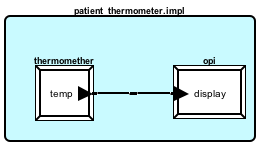
\includegraphics[height=1.5in]{figures/patient_thermometer.png}
    	\caption{AADL model of simple thermometer}
    \end{center}
    \label{figure:patient_thermometer}
\end{figure}

\singlespacing
\begin{lstlisting}[language=aadl, frame=single, gobble=0, caption={AADL model of simple thermometer}, label={listing:patient_thermometer}]
	package Thermometer
	public
	with Base_Types;
		system patient_thermometer
		end patient_thermometer;

		system implementation patient_thermometer.impl
		subcomponents
			thermomether : device thermometer_device.impl;
			opi : device operator_interface.impl;
		connections
			tdn : port thermomether.temp -> opi.display;
		end patient_thermometer.impl;

		device operator_interface
		features
			display : in data port Base_Types::Integer;
		end operator_interface;

		device implementation operator_interface.impl
		end operator_interface.impl;

		device thermometer_device
		features
			temp : out data port Base_Types::Integer;
		end thermometer_device;

		device implementation thermometer_device.impl
		end thermometer_device.impl;
	end Thermometer;
\end{lstlisting} 
\doublespacing
%another example: https://wiki.sei.cmu.edu/aadl/images/7/73/AADLV2Overview-AADLUserDay-Feb_2010.pdf (slide 16)

Recently AADL becomes a new market standard. There are lots of tools for AADL models analysis, such as: STOOD \footnote{http://www.ellidiss.com/products/stood}, ADELE \footnote{https://wiki.sei.cmu.edu/aadl/index.php/Adele}, Cheddar \footnote{http://beru.univ-brest.fr/~singhoff/cheddar}, AADLInspector \footnote{http://www.ellidiss.com/products/aadl-inspector} or Ocarina \footnote{http://www.openaadl.org}.

What is important, AADL is for architectural description. It should not be compared with UML suites, which allows to link with source code.


\subsection{OSATE}
\label{background:aadl:osate}
Open Source AADL Tool Environment (OSATE) is a set of plug-ins on top of the open-source Eclipse platform. It provides a toolset for front-end processing of AADL models. OSATE is developed mainly by SEI (Software Engineering Institute - CMU) \footnote{http://www.aadl.info/aadl/currentsite/tool/osate.html}. Latest available version of OSATE in the time when this work was published is OSATE2 \footnote{https://wiki.sei.cmu.edu/aadl/index.php/Osate\_2}.



\section{BLESS}
\label{background:bless}
BLESS (Behavior Language for Embedded Systems with Software) is AADL annex sublanguage defining behavior of components. The goal of BLESS is automatically-checked correctness proofs of AADL models of embedded electronic systems with software.

BLESS contains three AADL annex sublanguages:
\begin{itemize} \itemsep1pt \parskip0pt \parsep0pt
	\item Assertion - it can be attached individually to AADL features (e.g. ports)
	\item subBLESS - can be attached only to subprograms; it has only value transformations and Assertions without time expressions
	\item BLESS - it can be attached to AADL thread, device or system components; it contains states, transitions, timeouts, actions, events and Assertions with time expressions...
\end{itemize}

How it fits into the picture. Why it was developed. Corectness prove in AADL + behavior \cite{Bless:Paper}, from which we can generate SPARK Ada code.



\section{SPARK Ada}
\label{background:spark}

%http://www.cs.swan.ac.uk/~csetzer/lectures/critsys/09/critsysfinal2.pdf

First version of Ada programming language - Ada 83 - was designed to meet the US Department of Defence Requirements formalized in "Steelman" document \footnote{http://www.adahome.com/History/Steelman/steelman.htm}. Since that time, Ada evolved. There were Ada 95, Ada 2005 and Ada 2012 (released in December 10, 2012) \footnote{http://www.ada2012.org}. Ada is actively used in many Real-World projects\footnote{http://www.seas.gwu.edu/~mfeldman/ada-project-summary.html}, e.g. Aviation (Boeing \footnote{http://archive.adaic.com/projects/atwork/boeing.html}), Railway Transportation, Commercial Rockets, Satellites and even Banking. One of the main goals of Ada is to ensure software correctness and safety.

\begin{figure}[ht]%t=top, b=bottom, h=here
    \begin{center}
    	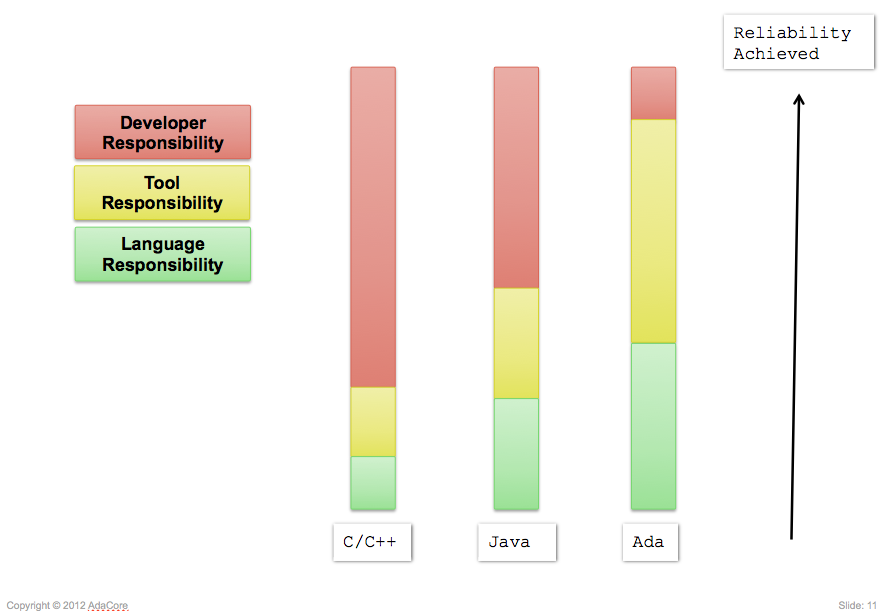
\includegraphics[height=3.5in]{figures/developer_responsibility_in_ada.png}
    	\caption{Developer responsibility in Ada\protect\footnotemark. }    	
    \end{center}
\end{figure}
\footnotetext{http://www.slideshare.net/AdaCore/ada-2012}

SPARK is a programming language and static verification technology designed specifically for the development of high integrity software. It is a "safe" subset of Ada designed to be susceptible to formal methods, accompanied with a set of approaches and tools. Using SPARK, a developer takes a Z specification and performs a stepwise refinement from the specification to SPARK code. For each refinement step a tool is used to produce verification conditions (VC's), which are mathematical theorems. If the VC's can be proved then the refinement step will be known to be valid. However if the VC's cannot be proved then the refinement step may be erroneous \footnote{http://www.dwheeler.com/lovelace/s17s4.htm}.

% Barnes' 15.7 where SPARK is used

First version was designed over 20 years ago. SPARK has established a track record of use in embedded and critical systems across a diverse range of industrial domains where safety and security are paramount \cite{Barnes:Book}. 

SPARK provides a significant degree of automation in proving exception freedom \cite{Spark:Article}. SPARK excludes some Ada constructs to make static analysis feasible \cite{Spark:Article}. Additionally SPARK contains tool-set for Software Verification:
\begin{itemize} \itemsep1pt \parskip0pt \parsep0pt
	\item Examiner - analyze code and ensures that it conforms to the SPARK language; also verify program to some extent using Verification Conditions (VC)
	\item Simplifier - simplify Verification Conditions generated by Examiner
	\item Proof Checker - prove the Verification Conditions
\end{itemize}

First version of SPARK was based on Ada 83. The second version (SPARK 95) - on Ada 95. SPARK 2005 is based on Ada 2005. It is a subset of Ada 2005 with annotations. The annotation language support flow analysis and formal verification. Annotations are encoded in Ada comments (via the prefix \lstinline{--#}). It makes every SPARK 2005 program, valid Ada 2005 program. Figure \ref{listing:Odometer2005} shows example SPARK 2005 package specification.

\singlespacing
\begin{lstlisting}[language=ada, frame=single, gobble=0, caption={SPARK 2005 code: Odometer \cite{Barnes:Book}}, label={listing:Odometer2005}]
	package Odometer
	--# own Trip, Total : Integer;
	is
		procedure Zero_Trip;
		--# global out Trip;
		--# derives Trip from ;
		--# post Trip = 0;

		function Read_Trip return Integer;
		--# global in Trip;

		function Read_Total return Integer;
		--# global in Total;

		procedure Inc;
		--# global in out Trip, Total;
		--# derives Trip from Trip & Total from Total;
		--# post Trip = Trip~ + 1 and Total = Total~ + 1;

	end Odometer;
\end{lstlisting} 
\doublespacing

SPARK 2005 does not include constructs such as pointers, dynamic memory allocation or recursion \cite{Spark:Article}.

SPARK 2014 \footnote{http://www.spark-2014.org} is based on Ada 2012 programming language targeted at safety- and security-critical applications \cite{Spark2014:Paper}. Since Ada 2012 contains contracts, there is no need to use annotations like in SPARK 2005. Thus SPARK 2014 is subset of Ada 2012. It contains all features of Ada 2012 except:
\begin{itemize} \itemsep1pt \parskip0pt \parsep0pt
 	\item Access types (pointers)
 	\item Exceptions
	\item Aliasing between variables
	\item Concurrency features of Ada (Tasking) - it's part of SPARK 2014 road-map to include support for tasking in the future, although likely not this year
	\item Side effects in expressions and functions
\end{itemize}

Sample mapping from SPARK 2005 to 2014 is shown on table \ref{table:spark2005and2014mapping}. Complete mapping can be found in SPARK 2014 documentation \footnote{http://docs.adacore.com/spark2014-docs/html/lrm/mapping-spec.html} \cite{Spark2014refManual:Online}.

\singlespacing
\begin{table}[!ht]
	\caption{Sample SPARK 2005 to 2014 mapping.}
	\label{table:spark2005and2014mapping}
	\centering
  	\begin{tabular}{ | p{3in} | p{3in} |}
	  	%\multicolumn{1}{c}{\textbf{AADL/BLESS}} & \textbf{SPARK Ada}\\

		\hline
		\multicolumn{1}{|c|}{\textbf{SPARK 2005}} & \multicolumn{1}{|c|}{\textbf{SPARK 2014}} \\ \hline

		\begin{lstlisting}
			--# global in out X, Y;
		\end{lstlisting} 
		& 
		\begin{lstlisting}[language=ada2012]
			with Global  => (In_Out => (X, Y));
		\end{lstlisting} 

		\\ \hline

		\begin{lstlisting}
			--# derives X from Y &
			--#         Y from X;
		\end{lstlisting} 
		& 
		\begin{lstlisting}[language=ada2012]
			Depends => (X => Y,
			            Y => X);
		\end{lstlisting}

		\\ \hline

		\begin{lstlisting}
			--# pre Y /= 0 and
			--#     X > Integer'First;
		\end{lstlisting} 
		& 
		\begin{lstlisting}[language=ada2012]
			with Pre  => Y /= 0 and 
			             X > Integer'First;
		\end{lstlisting}

		\\ \hline

		\begin{lstlisting}
			--# post X = Y~ and Y = X~;
		\end{lstlisting} 
		& 
		\begin{lstlisting}[language=ada2012]
			with Post => (X = Y'Old and Y = X'Old);
		\end{lstlisting} 

		\\ \hline
	\end{tabular}
\end{table}
\doublespacing

SPARK 2014 does not contains Examiner. Instead, proofs are made by gnatPROVE.
The notion of executable contracts in Ada 2012, was inspired by SPARK. The previous Odometer example in SPARK 2014 is shown in figure \ref{listing:Odometer2014}.

\singlespacing
\begin{lstlisting}[language=ada2012, frame=single, gobble=0, caption={SPARK 2014 code: Odometer}, label={listing:Odometer2014}]
	package Odometer
	with SPARK_Mode
	Abstract_State => (Trip, Total)
	is
		procedure Zero_Trip
		with Global => (Output => (Trip)),
		   Depends => (Trip => null),
		   Post => (Trip = 0);

		function Read_Trip return Integer
		with Global => (Input => (Trip));

		function Read_Total return Integer
		with Global => (Input => (Total));

		procedure Inc	   
		with Global => (In_Out => (Trip, Total)),
			Depends => (Trip => Trip, Total => Total),
			Post => Trip = Trip'Old + 1 and Total = Total'Old + 1;

	end Odometer;
\end{lstlisting} 
\doublespacing

Fundamental SPARK contracts:

\singlespacing
\begin{center}
	\begin{longtable}{| p{1.5in} | p{1.5in} | p{3in} |}
		\caption{Fundamental SPARK annotations}
		\label{table:SparkAnnotations}
		\\
		\hline
		\multicolumn{1}{|c|}{\textbf{SPARK 2005}} & \multicolumn{1}{|c|}{\textbf{SPARK 2014}} & \multicolumn{1}{|c|}{\textbf{Description}} \\ \hline
		\endfirsthead

		\multicolumn{3}{c}%
		{{\bfseries \tablename\ \thetable{} -- continued from previous page}} \\
		\hline 
		\multicolumn{1}{|c|}{\textbf{SPARK 2005}} & \multicolumn{1}{|c|}{\textbf{SPARK 2014}} & \multicolumn{1}{|c|}{\textbf{Description}} \\ \hline
		\endhead

		\hline \multicolumn{3}{|r|}{{Continued on next page}} \\ \hline
		\endfoot

		\hline %\hline
		\endlastfoot

		\begin{lstlisting}
			--# global
		\end{lstlisting} 
		& 
		\begin{lstlisting}[language=ada2012]
			Global
		\end{lstlisting} 
		& 
		list of used global variables within subprogram 

		\\ \hline

		\begin{lstlisting}
			--# derives
		\end{lstlisting} 
		& 
		\begin{lstlisting}[language=ada2012]
			Depends
		\end{lstlisting} 
		& 
		describe dependencies between variables

		\\ \hline

		\begin{lstlisting}
			--# own 
		\end{lstlisting} 
		& 
		\begin{lstlisting}[language=ada2012]
			Abstract_State
		\end{lstlisting} 
		& 
		declare variables defined in package body

		\\ \hline

		\begin{lstlisting}
			--# initializes
		\end{lstlisting} 
		& 
		\begin{lstlisting}[language=ada2012]
			initializes
		\end{lstlisting} 
		& 
		indicates variables, which are initialized

		\\ \hline

		\begin{lstlisting}
			--# inherit
		\end{lstlisting} 
		& 
		not needed
		& 
		allows to access entities of other packages

		\\ \hline

		\begin{lstlisting}
			--# pre
		\end{lstlisting} 
		& 
		\begin{lstlisting}[language=ada2012]
			Pre
		\end{lstlisting} 
		& 
		pre condition

		\\ \hline
		

		\begin{lstlisting}
			--# post
		\end{lstlisting} 
		& 
		\begin{lstlisting}[language=ada2012]
			Post
		\end{lstlisting} 
		& 
		post condition

		\\ \hline
		

		\begin{lstlisting}
			--# assert
		\end{lstlisting} 
		& 
		\begin{lstlisting}[language=ada2012]
			Assert
		\end{lstlisting} 
		& 
		assertion

		\\ \hline
	\end{longtable}
\end{center}
\doublespacing

It is possible to mix SPARK 2014 with Ada 2012. However, only the part which is SPARK 2014 compliant will be verified. Usually SPARK is used in the most critical parts of Software Systems \cite{Spark:IndustrialExp}. It means, that some part is written in e.g. Ada or C++ and the rest in SPARK. The reason of that is the SPARK limitation and lack of necessity to verify some modules.
% http://docs.adacore.com/spark2014-docs/html/ug/spark_2014.html#mixing-spark-code-and-ada-code

The most popular IDE for SPARK Ada is GNAT Programming Studio \footnote{http://libre.adacore.com/tools/gps}.

There is also plugin for Eclipse: GNATbench \footnote{https://www.adacore.com/gnatpro/toolsuite/gnatbench/} created by AdaCore. 
Tools for correctness proving.


\subsection{GNAT compiler and Programming Studio}
\label{background:spark:gps}
GNAT compiler is front end of gcc...
IDE for SPARK Ada programs development. Includes proving tools. E.g. Sireum Bakar (developed by SAnToS lab) or GNATprove.


\subsection{Ravenscar Tasking Subset}
\label{background:spark:ravenscar}

RavenSPARK is subset of the SPARK Ravenscar Profile (which is subset of Ada tasking). The Ravenscar Profile provides a subset of the tasking facilities of Ada95 and Ada 2005 suitable for the construction of high-integrity concurrent programs \cite{Ravenscar:Online}.

The Ravenscar Profile is a subset of the tasking model, restricted to meet the real-time community requirements for determinism, schedulability analysis and memory-boundedness, as well as being suitable for mapping to a small and efficient run-time system that supports task synchronization and communication, and which could be certifiable to the highest integrity levels. The concurrency model promoted by the Ravenscar Profile is consistent with the use of tools that allow the static properties of programs to be verified. Potential verification techniques include information flow analysis, schedulability analysis, execution-order analysis and model checking. These techniques allow analysis of a system to be performed throughout its development life cycle, thus avoiding the common problem of finding only during system integration and testing that the design fails to meet its non-functional requirements. \cite{Ravenscar:Article}

Concurrent programs require the use of different specification and verification techniques from sequential programs. For this reason, tasks, protected units and objects, and synchronization features are currently excluded from SPARK 2014 \footnote{http://docs.adacore.com/spark2014-docs/html/lrm/tasks-and-synchronization.html} \cite{Spark2014refManual:Online}.

To create a task, the task type has to be declared and task variable of this type. Ravenscar does not allow dynamic task creation. Thus, all tasks have to exists for the full lifetime of the program. \cite{IssuesWithRavenscar:Paper} Tasks can be declared only in packages. Not in subprograms or in other tasks. \cite{Barnes:Book} The priority of each tasks has to be specified by \lstinline{pragma Priority}. [what is priorities range?] Listing \ref{lst:SampleTask} shows sample package with two tasks.

\singlespacing
\begin{lstlisting}[frame=single, gobble=0, caption={Sample tasks}, label={lst:SampleTask}]
	package Some_Pkg
	--# own task t1 : Task1;
	--#     task t2 : Task2;
	is
		task type Task1
		is
			pragma Priority(10);
		end Task1;

		task type Task2
		is
			pragma Priority(9);
		end Task2;

	end Some_Pkg;
\end{lstlisting} 
\doublespacing

Declared tasks have to be implemented in the package body (listing \ref{lst:SampleTaskBody}).

\singlespacing
\begin{lstlisting}[frame=single, gobble=0, caption={Sample tasks body}, label={lst:SampleTaskBody}]
	package body Some_Pkg
	is
		t1 : Task1;
		t2 : Task2;

		task body Task1
		is
		begin
			loop
				-- implementation;
			end loop;
		end Task1;

		task body Task2
		is
		begin
			loop
				-- implementation;
			end loop;
		end Task2;

	end Some_Pkg;
\end{lstlisting} 
\doublespacing

There are two ways to access variable in different tasks:
\begin{itemize}
    \item It has to be protected object
    \item It has to be atomic type
\end{itemize}


Protected object encapsulate variable, in such a way that it is accessible, only through protected subprograms. This mechanism use locking, to ensure atomicity. Protected type declaration is similar to task: specification and body has to be defined. Listing \ref{lst:SampleTasksWithProtectedType} shows sample tasks with protected type \lstinline{Integer_Store}, which enable to share Integer variable between tasks. What is important, protected type has to be declared before tasks, which will use it. Otherwise, it will not be visible for them.

\singlespacing
\begin{lstlisting}[frame=single, gobble=0, caption={Sample tasks with protected object}, label={lst:SampleTasksWithProtectedType}]
	package Some_Pkg
	--# own protected Shared_Var : Integer_Store (Priority => 11);
	--#     task t1 : Task1;
	--#     task t2 : Task2;
	is
	    protected type Integer_Store
	    is
	        pragma Priority (11);

	        function Get return Integer;
	        --# global in Integer_Store;

	        procedure Put(X : in Integer);
	        --# global out Integer_Store;
	        --# derives Integer_Store from X;
	    private
	        TheStoredData : Integer := 0;
	    end Integer_Store;

	    task type Task1
	      --# global out Shared_Var;
	    is
	        pragma Priority(10);
	    end Task1;

	    task type Task2
	      --# global in Shared_Var;
	    is
	        pragma Priority(9);
	    end Task2;

	end Some_Pkg;
\end{lstlisting}
\doublespacing

Protected type body also has to be defined in package body (listing \ref{lst:SampleTasksWithProtectedTypeBody}).

\singlespacing
\begin{lstlisting}[frame=single, gobble=0, caption={Sample tasks with protected object body}, label={lst:SampleTasksWithProtectedTypeBody}]
	package body Some_Pkg
	is
	    Shared_Var : Integer_Store;
	    t1 : Task1;
	    t2 : Task2;

	    protected body Integer_Store is
	        function Get return Integer
	        --# global in TheStoredData;
	        is
	        begin
	            return TheStoredData;
	        end Get;

	        procedure Put(X : in Integer)
	        --# global out TheStoredData;
	        --# derives TheStoredData from X;
	        is
	        begin
	            TheStoredData := X;
	        end Put;
	    end Integer_Store;

	    task body Task1
	    is
	    begin
	        loop
	            Shared_Var.Put(5);
	        end loop;
	    end Task1;

	    task body Task2
	    is
	        Local_Var : Integer;
	    begin
	        loop
	            Local_Var := Shared_Var.Get;
	        end loop;
	    end Task2;

	end Some_Pkg;
\end{lstlisting} 
\doublespacing

\lstinline{Task1} is writing to \lstinline{Shared_Var} and \lstinline{Task2} is reading \lstinline{Shared_Var}. The highest priority is assigned to protected object, to ensure atomicity during operations on it. The lowest priority is assigned to \lstinline{Task2}, which is reading \lstinline{Shared_Var}. Reading is usually less expensive operation than writing. Thus, to avoid starvation, \lstinline{Task1} has higher priority than \lstinline{Task2}. Notice, that \lstinline{Shared_Var} is declared in package body, but refined in package specification.

Protected variables may not be used in proof contexts. Thus, if we try to use protected variable in proofs (pre- or postcondition), then SPARK Examiner returns \lstinline{Semantic Error 940 - Variable is a protected own variable. Protected variables may not be used in proof contexts.}. Formal reasoning about interactions and especially temporal properties require other techniques such as model checking and lie outside the scope of SPARK \cite{Barnes:Book}. To preserve opportunity to use pre- and postconditions, atomic types have to be used.

To declare atomic type, we have to use \lstinline{pragma Atomic}. However, there is restriction, that \lstinline{pragma Atomic} cannot be applied to predefined type such as Integer. Thus, we have to define our custom type (which can be just rename of Integer) and apply \lstinline{pragma Atomic} on this type. Listing \ref{lst:SampleTasksWithAtomicType} presents previous example with atomic types instead of protected objects.

\singlespacing
\begin{lstlisting}[frame=single, gobble=0, caption={Sample tasks with atomic type}, label={lst:SampleTasksWithAtomicType}]
	package Some_Pkg
	--# own Shared_Var;
	--#     task t1 : Task1;
	--#     task t2 : Task2;
	--# initializes Shared_Var;
	is
	    type Int32 is new Integer;
	    
	    task type Task1
	      --# global out Shared_Var;
	    is
	        pragma Priority(10);
	    end Task1;

	    task type Task2
	      --# global in Shared_Var;
	    is
	        pragma Priority(9);
	    end Task2;

	end Some_Pkg;

	package body Some_Pkg
	is    
	    Shared_Var : Int32 := 0;
	    t1 : Task1;
	    t2 : Task2;

	    task body Task1
	    is
	    begin
	        loop
	            Shared_Var := 5;
	        end loop;
	    end Task1;

	    task body Task2
	    is
	        Local_Var : Integer;
	    begin
	        loop
	            Local_Var := Integer(Shared_Var);
	        end loop;
	    end Task2;

	end Some_Pkg;
\end{lstlisting}
\doublespacing

Be aware that \lstinline{pragma atomic} does not guaranty atomicity. In most cases, atomic types should not be used for tasking. Instead, protected types should be used.
% precise! http://en.wikibooks.org/wiki/Ada_Programming/Pragmas/Atomic

Another important thing in tasking is Time library: \lstinline{Ada.Real_Time}. It allows to run task periodically, using \lstinline{delay until} statement, which suspends task until specified time. To use \lstinline{delay} in the task, it has to be declared in \lstinline{declare} annotation: \lstinline{--# declare delay;} \cite{Barnes:Book}.

Details about tasking in SPARK are well described in Chapter 8 of Barnes' book \cite{Barnes:Book}. The "Guide for the use of the Ada Ravenscar profile in high integrity systems" \cite{Ravenscar:Article} and the official Ravenscar Profile documentation (which includes examples) \cite{Ravenscar:Online} might be useful as well. The limitations of Tasking in SPARK are reviewed in Audsley's and Welllings' paper \cite{IssuesWithRavenscar:Paper}.


\section{SPARK Ada Verification}
\label{background:sparkverification}

%http://docs.adacore.com/sparkdocs-docs/

Verification - what is that
verification vs validation

SPARK tools
FDL is the modelling language of the SPARK proof tools. 

\begin{figure}[ht]%t=top, b=bottom, h=here
    \begin{center}
    	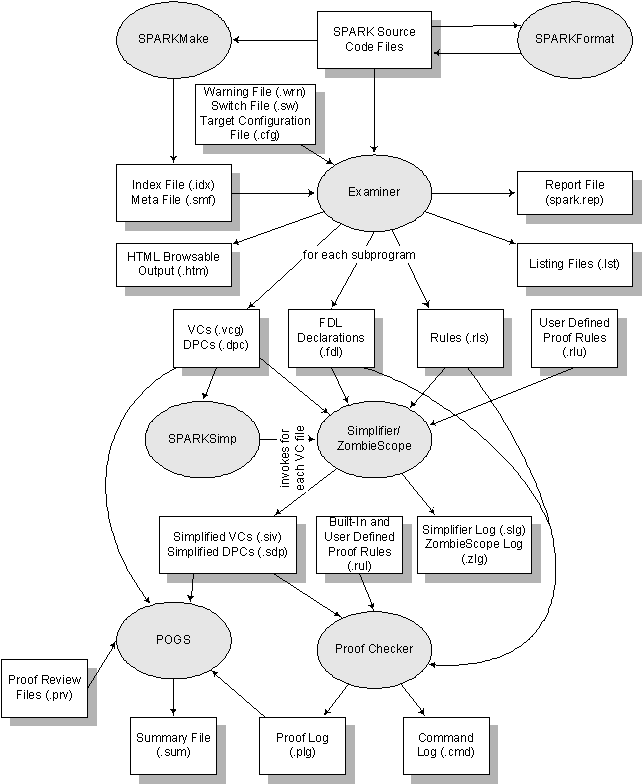
\includegraphics[height=7in]{figures/spark-tools.png}
    	\caption{Relationship of the Examiner and Proof Tools\protect\footnotemark.}
    \end{center}
\end{figure}
\footnotetext{http://docs.adacore.com/sparkdocs\-docs/Examiner\_UM.htm}



\subsection{SPARK Examiner}
\label{verification:examiner}

The main SPARK verification tool is Examiner. It supports several levels of analysis:
\begin{itemize}
	\item checking of SPARK language syntactic and static semantic rules
	\item data flow analysis
	\item data and information flow analysis
	\item formal program verification via generation of verification conditions
	\item proof of absence of run-time errors
	\item dead path analysis
\end{itemize}

There is also an option to make the Examiner perform syntax checks only. Using this option on a source file does not require access to any other units on which the file depends, so files can be syntax checked on an individual basis. This allows any syntax errors to be corrected before the file is included in a complex examination.  This option must only be used as a pre-processor: the absence of syntax errors does NOT indicate that the source text is a legal SPARK program. \cite{Examiner:Online} (THIS PART IS COPY AND PASTE FROM Examiner doc - is it ok?)

Put here some examples: method without contract, examine, add specification, pass Examiner.

During implementation, code was regularly checked using SPARK Examiner.

What is very important, Examiner can perform data and information analysis of Ravenscar programs in exactly the same manner as for sequential programs \cite{Ravenscar:Online}. Unfortunately it does not allow protected objects in proof annotations (pre- and post-conditions).

When some parts of the system are written in full Ada (with non-valid SPARK constructs), then Examiner returns error. Ada parts can be excluded from Examiner analysis using \lstinline{--# hide} annotation. The, only warning \lstinline{10 - The body of subprogram Main is hidden - hidden text is ignored by the Examiner.} is returned by Examiner.

Examiner use SPARK index file to locate files necessary for verification. \cite{Barnes:Book}

Examiner can be used with \lstinline{spark} command and appropriate flags described in Examiner Manual \cite{Examiner:Online}.

%http://docs.adacore.com/sparkdocs-docs/SPARK_GPS.htm
%[screenshot - take from 721 paper]
To use Examiner in GNAT Programming Studio:
\begin{itemize}
	\item Run SPARK Make (right click on project / SPARK / SPARK Make)
	\item Set SPARK index file (to spark.idx generated by SPARKMake) [add photo from 721 paper]
	\item (optionally) set configuration file (Standard.ads)
	\item Choose appropriate version of SPARK (95 or 2005)
	\item Choose mode: Sequential (for single tasking programs) or Ravenscar (for multitasking programs)
\end{itemize}

To generate verification conditions (VCs), the \lstinline{-vcg} switch has to be used. It can be set in GNAT Programming Studio (Project / Edit project properties / Switches / Examiner / Generate VCs).
In addition to verification conditions, Examiner can check dead path conjectures. It checks, whether all of the program is useful. To generate dead path conjectures, the \lstinline{-dpc} switch has to be used. It can be also set in GNAT Programming Studio (Project / Edit project properties / Switches / Examiner / Generate DPCs).


\subsubsection{Flow analysis}
\label{verification:examiner:flowanalysis}
%http://www.cs.swan.ac.uk/~csetzer/lectures/critsys/09/critsysfinal2.pdf
There are two types of flow analysis:
\begin{itemize}
	\item Data flow analysis:
	\begin{itemize}
		\item Checks input/output behavior of parameters and variables.
		\item Checks initialization of variables.
		\item Checks that changed and imported variables are used later (possibly as output variables).
	\end{itemize}
	\item Information flow analysis - verifies interdependencies between variables.
\end{itemize}

In data flow analysis, Examiner checks if input parameters are not modified, but used at least once (in at least one branch of program). In the same factor, output parameters cannot be read (before initialization) and has to be initialized (in all branches of program). Input/output parameters has to be both read and write (changed). In similar way, Examiner verify the global variables (specified in annotations). Functions can use only input parameters and can only read global variables. Therefore functions do not have side effects. 

Global variables defined in package body (thus private) has to be declared by \lstinline{--# own} annotation in package specification. If variable is also initialized, \lstinline{--# initializes} annotation has to be used. In Ada, to use package in another package, \lstinline{with} clause has to be used. In SPARK Ada, additionally \lstinline{--# inherits} annotation has to be specified.

In information flow analysis, dependencies between variables are analyzed. These dependencies are specified by \lstinline{--# derives} annotation.


\subsubsection{Verification conditions}
\label{verification:examiner:vc}

To generate verification conditions, two kinds of annotations are relevant for Examiner:
\begin{itemize}
	\item pre-conditions: \lstinline{--# pre}
	\item post-conditions: \lstinline{--# post}
\end{itemize}

Notion of pre- and post-conditions represents Hoare logic. More precisely, Hoare triple: 

\begin{equation} \label{eq:hoare_triple}
	\{P\} C \{Q\}
\end{equation}

P and Q are assertions. C is a command (action) performed between them. P is pre-condition and Q is post-condition.

Additionally, assertions (\lstinline{--# assert}) and checks (\lstinline{--# check}) can be specified in procedure body. Then additional verification conditions are generated.

Functions does not have side effects (as stated in \ref{verification:examiner:flowanalysis}), thus only pre-condition can be applied. However, there is annotation \lstinline{--# return}, which specify function return value.

Verification conditions are generated depended on number of paths in subprogram. Analysis are perform backwards, in other words: we start from post-conditions and consider what must holds before. Flow analysis is well described in chapter 11 of Barnes' book \cite{Barnes:Book}.



\subsection{SPARK Simplifier}
\label{verification:simplifier}

Simplifier can discharge (prove correctness) of verification conditions (VCs) generated by Examiner, but not proved by Examiner. \cite{Simplifier:Online} 



\subsection{ZombieScope}
\label{verification:zombiescope}

ZombieScope is a SPARK tool, that analyses SPARK code to find dead paths, i.e. paths through the code that can never be executed.


\subsection{Victor}
\label{verification:victor}

Victor is a tool to translate SPARK verification conditions (VCs), as generated by the Examiner, into SMT-LIB (file format used to communicate with SMT solvers). \cite{Victor:Online} SMT (Satisfiability Modulo Theories) solver is a tool...
experimental feature
Integrated with SPARKSimp (by -victor flag) and POGS.


\subsection{Proof Checker}
\label{verification:proofchecker}

% Barnes' book: 12.12
Only mention. It is hardcore.

\subsection{SPARKSimp Utility}
\label{verification:sparksimp}
SPARKSimp is a simple "make" style tool for the SPARK analysis tools. Currently, it supports the Simplifier, ZombieScope and ViCToR. It applies the Simplifier (and ViCToR, if requested, please see the Victor\_Wrapper user manual \cite{Victor:Online} for more information) to all .vcg files and ZombieScope to all .dpc files it finds in a directory tree. \cite{SPARKSimp:Online} 



\subsection{Proof Obligation Summarizer (POGS)}
\label{verification:pogs}

The Proof ObliGation Summarizer tool (POGS) reads and understands the structure of the verification condition files. It reports the status of proofs and dead path analyses in a human-readable form. \cite{POGS:Online}

\subsection{AUnit}
\label{background:spark:aunit}
AUnit is Unit Test Framework for Ada language. It can be also applied for verify SPARK Ada programs.
AUnit tutorials \cite{AUnitTutorials:Online}
AUnit Cookbook \cite{AUnitCookbook:Online}


\subsection{Sireum Bakar}
\label{background:spark:sireum}
Overview: symbolic execution, Pilar, Kiasan and Alir \cite{Hari:Thesis}.
Sireum Kiasan \cite{Kiasan:Paper} is a tool, which use symbolic execution for finding possible paths in program.
Plugin for GNAT Programming Studio (SPARK 2005 and 2014 under development).
Plugin for Eclipse (only for SPARK 2005).
No support for Ravenscar profile.
Separated sequential parts can be verified (Odometer?). Sequential version of \lstinline{Max_Drug_Per_Hour_Watcher}?


\subsection{GNAT Prove}
\label{background:spark:gnatprove}
GNATprove \footnote{http://www.open-do.org/projects/hi-lite/gnatprove/} is a formal verification tool for SPARK 2014 programs. It interprets SPARK Ada annotations exactly like they are interpreted at run time during tests.
% http://docs.adacore.com/spark2014-docs/html/ug/gnatprove.html
% only for SPARK 2014


\section{AADL/BLESS to SPARK Ada code generation}
\label{background:codegen}
The ultimate goal of long term research, this thesis is part of, is AADL (with BLESS) to SPARK Ada translation.


\subsection{Ocarina}
\label{background:codegen:ocarina}
Ocarina \cite{Ocarina:Paper,Ocarina:Paper} generates code from an AADL architecture model to an Ada application running on top of PolyORB framework. In this context, PolyORB acts as both the distribution middleware and execution runtime on all targets supported by PolyORB.
It generate Ada 2005 and C code.
Since mid-2009, Telecom ParisTech is no longer involved in Ocarina, and is developing another AADL tool-chain, based on Eclipse, codenamed RAMSES \cite{Ocarina:About:Online}.

examples on github

run:
ocarina -x scenario.aadl



\subsection{Ramses}
\label{background:codegen:ramses}
% very shortly
RAMSES is a model transformation framework dedicated to the refinement of AADL models. It contains code generation plug-in.
% http://www.aadl.info/aadl/downloads/committee/feb2013/presentations/RAMSES_status_2013_06_02_format.pdf
% https://wiki.sei.cmu.edu/aadl/index.php/OSATE_2_on_the_command-line
%!TEX root = etdrtemplate.tex
% +--------------------------------------------------------------------+
% | Sample Chapter 3
% +--------------------------------------------------------------------+

\cleardoublepage

% +--------------------------------------------------------------------+
% | Replace "This is Chapter 3" below with the title of your chapter.
% | LaTeX will automatically number the chapters.
% +--------------------------------------------------------------------+

\chapter{PCA Pump Prototype}
\label{pcapump}

Overview of PCA Pump and issues, which MDCF/ICE will solve.
In this thesis, only the operation module is implemented.


\section{PCA Pump Requirements Document}
\label{pcapump:requirements-doc}
Selected use cases for implementation?
Overview of issues solved: 
* Bolus options: FBasal + FPatient or FPatient


\section{PCA Pump AADL/BLESS Models}
\label{pcapump:aadl-bless-models}
Selected modules for implementation. Pictures etc.


\section{BeagleBoard-XM}
\label{pcapump:beagleboard}
First step was create PCA Pump prototype on BeagleBoard-xM.

BeagleBoard-xM is Embedded device with AM37x 1GHz ARM processor (Cortex-A8 compatible). It has 512 MB RAM, 4 USB 2.0 ports, HDMI port, 28 General-purpose input/output (GPIO) ports and Linux Operating System (on microSD card). All these properties makes this device good candidate for prototyping PCA Pump.

Expansion port 14 and 28
GPIO158
Java Program to Run the pump for 10 seconds

There is no existing SPARK/Ada compiler running on ARM system. Hence, to compile SPARK/Ada program for ARM device, we need to perform cross-compilation on other machine. There is GNAT compiler \cite{Horn:Thesis} created by AdaCore, but there was no cross-compiler for ARM. However AdaCore was working on it. They had working version in 2013, but tested only on their target, Android-based device. BeagleBoard-xM is coming with Linux Angstrom Operating System. There is possibility to install Android on BeagleBoard-xM, but still not warranty everything will be working. Cooperation with AdaCore allowed to cross-compile SPARK/Ada program for BeagleBoard-xM.

Include source of simple program?
GNAT cross-compiler only for Linux Platform (cross-compilation has to be done on Linux).


\section{PCA Pump Prototype Implementation}
\label{pcapump:implementation}

Currently SPARK 2014 does not support tasking \cite{Spark2014refManual:Online}. For SPARK 2005, GNAT compiler provides Ravenscar Profile \cite{Ravenscar:Online}. It provides a subset of the tasking facilities of Ada95 and Ada 2005 suitable for the construction of high-integrity concurrent programs.

Issues: Ravenscar Profile, how to deal with different boluses (look at UMinn requirements and annotations for our doc).
Look at annotated PCA Pump Req document.

\subsection{Concurrency in SPARK}
\label{pcapump:implementation:concurrency}

Concurrent programs require the use of different specification and verification techniques from sequential programs. For this reason, tasks, protected units and objects, and synchronization features are currently excluded from SPARK 2014 \footnote{http://docs.adacore.com/spark2014-docs/html/lrm/tasks-and-synchronization.html} \cite{Spark2014refManual:Online}.

In SPARK 2005, concurrency is enable using the Ravenscar profile \cite{Ravenscar:Online}. 

\cite{Ravenscar:Article}

\subsection{Interface for Integrated Clinical Environment}
\label{pcapump:implementation:ice}

Describe communication with MDCF/ICE. PCA Pump ports for that etc.
%!TEX root = etdrtemplate.tex
% +--------------------------------------------------------------------+
% | Sample Chapter 4
% +--------------------------------------------------------------------+

\cleardoublepage

% +--------------------------------------------------------------------+
% | Replace "This is Chapter 4" below with the title of your chapter.
% | LaTeX will automatically number the chapters.
% +--------------------------------------------------------------------+

\chapter{AADL/BLESS to SPARK/Ada translation}
\label{codegen}

First step was to create mock (based on doc, aadl models and implemented PCA Pump).
Prototyping Embedded Systems using AADL lasts for a few years \cite{PrototypyingAadl:Paper}.

\section{AADL/BLESS to SPARK/Ada mapping}
\label{codegen:mapping}

%https://wiki.sei.cmu.edu/aadl/images/4/40/13_04_24-AADL-Code_Generation.pdf

%https://wiki.sei.cmu.edu/aadl/images/7/73/AADLV2Overview-AADLUserDay-Feb_2010.pdf (slide 35: port connections)

Mapping is driven by "Architecture analysis \& Design Language (AADL) V2 Programming Language Annex Document" \cite{AnnexDoc13}. Ocarina tool suite (based on older AADL annex documents \cite{Ocarina:Article}) was also helpful in understanding of AADL to Ada translation.
Only high level mapping is done. No implementation (thread interactions) like Ocarina does. 

3 areas of mapping:
* data types
* thread -> subprograms
* subprogram -> subprogram

\subsection{Data types mapping}
\label{codegen:mapping:data}

\subsection{AADL ports mapping}
\label{codegen:mapping:ports}

Proposed ports mapping shown in table \ref{table:aadl2spark_ports} is based on AADL runtime services from Annex 2 to "Programming Language Annex Document" \cite{AnnexDoc13}.

% maybe split right column into 2 rows: spec and body?
\begin{center}
	\begin{longtable}{| p{2in} | p{4in} |}
	
		\caption{AADL to SPARK ports mapping.}
		\label{table:aadl2spark_ports}
		\\
		\hline
		\multicolumn{1}{|c|}{\textbf{AADL/BLESS}} & \multicolumn{1}{|c|}{\textbf{SPARK/Ada}} \\ \hline
		\endfirsthead

		\multicolumn{2}{c}%
		{{\bfseries \tablename\ \thetable{} -- continued from previous page}} \\
		\hline 
		\multicolumn{1}{|c|}{\textbf{AADL/BLESS}} & \multicolumn{1}{|c|}{\textbf{SPARK/Ada}} \\ \hline
		\endhead

		\hline \multicolumn{2}{|r|}{{Continued on next page}} \\ \hline
		\endfoot

		\hline %\hline
		\endlastfoot

		\begin{lstlisting}[language=aadl]
			Port_Name : 
				in data port Port_Type;
		\end{lstlisting} 
		&
		\begin{lstlisting}[language=ada]
			-- spec (.ads):
			procedure Receive_Port_Name;

			-- body (.adb):
			Port_Name : Port_Type;

			procedure Receive_Port_Name 
			is
			begin
				-- TODO: implement receiving Port_Name value
				-- e.g.:
				-- Port_Name := Some_Pkg.Get_Port_Name;
			end Receive_Port_Name;
		\end{lstlisting} 

		\\ \hline

		\begin{lstlisting}[language=aadl]
			Port_Name : 
				out data port Port_Type;
		\end{lstlisting} 
		&
		\begin{lstlisting}[language=ada]
			-- spec (.ads)
			function Get_Port_Name : Port_Type;

			-- body (.adb):
			Port_Name : Port_Type;

			function Get_Port_Name : Port_Type 
			is
			begin
				return Port_Name;
			end Get_Port_Name;
		\end{lstlisting} 

		\\ \hline

		\begin{lstlisting}[language=aadl]
			Port_Name : 
				in event port;
		\end{lstlisting} 
		&
		\begin{lstlisting}[language=ada]
			-- spec (.ads)
			procedure Put_Port_Name(Port_Name_In : Boolean);

			-- body (.adb):
			Port_Name : Boolean;

			procedure Put_Port_Name (Port_Name_In : Boolean) 
			is
			begin
				Port_Name := Port_Name_In;
			end Put_Port_Name;
		\end{lstlisting} 

		\\ \hline

		\begin{lstlisting}[language=aadl]
			Port_Name : 
				out event port;
		\end{lstlisting} 
		&
		\begin{lstlisting}[language=ada]
			-- spec (.ads)
			procedure Send_Port_Name;

			-- body (.adb):
			Port_Name : Boolean;

			procedure Send_Port_Name 
			is
			begin
				-- TODO: implement receiving Port_Name value
				-- e.g.:
				-- Port_Name := Some_Pkg.Put_Port_Name(Port_Name);
			end Send_Port_Name;
		\end{lstlisting} 

		\\ \hline

		\begin{lstlisting}[language=aadl]
			Port_Name : 
				in event data port Port_Type;
		\end{lstlisting} 
		&
		\begin{lstlisting}[language=ada]
			-- spec (.ads)
			procedure Put_Port_Name(Port_Name_In : Port_Type);

			-- body (.adb):
			Port_Name : Port_Type;

			procedure Put_Port_Name (Port_Name_In : Port_Type) 
			is
			begin
				Port_Name := Port_Name_In;
			end Put_Port_Name;
		\end{lstlisting} 

		\\ \hline

		\begin{lstlisting}[language=aadl]
			Port_Name : 
				out event data port Port_Type;
		\end{lstlisting} 
		&
		\begin{lstlisting}[language=ada]
			-- spec (.ads)
			procedure Send_Port_Name;

			-- body (.adb):
			Port_Name : Port_Type;

			procedure Send_Port_Name 
			is
			begin
				-- TODO: implement receiving Port_Name value
				-- e.g.:
				-- Port_Name := Some_Pkg.Put_Port_Name(Port_Name);
			end Send_Port_Name;
		\end{lstlisting} 
	\end{longtable}
\end{center}


\subsection{Thread to subprograms mapping}
\label{codegen:mapping:threads}

AADL package, which contains threads is split into child packages with convention: AADL\_Package\_Name -> AADL\_Package\_Name.Thread\_Name.

In SPARK/Ada we have nested packages and child packages. Sample nested packages are shown in listing \ref{listing:nested_packages}. Equivalent child packages are shown in listing \ref{listing:child_packages}. The name of a child package consists of the parent unit's name followed by the child package's identifier, separated by a period (dot) `.'. Calling convention is the same for child and nested packages (e.g. \lstinline{P.N} in listings \ref{listing:nested_packages} and \ref{listing:child_packages}. However, there is a difference between nested packages and child packages. In nested package declarations become visible as they are introduced, in textual order. For example, in listing \ref{listing:nested_packages} spec \lstinline{N} cannot refer to \lstinline{M} in any way. In case of child packages, with certain exceptions, all the functionality of the parent is available to a child and parent can access all its child packages. More precisely: all public and private declarations of the parent package are visible to all child packages. Private child package can be accessed only from parent's body.

\begin{lstlisting}[language=ada, frame=single, gobble=0, caption={Nested packages in SPARK/Ada}, label={listing:nested_packages}]
	package P is
	   D: Integer;

	   --  a nested package:
	   package N is
	      X: Integer;
	   private
	      Foo: Integer;
	   end N;

	   E: Integer;
	private
	   --  nested package in private section:
	   package M is
	      Y: Integer;
	   private
	      Bar: Integer;
	   end M;

	end P;
\end{lstlisting}

\begin{lstlisting}[language=ada, frame=single, gobble=0, caption={Child packages in SPARK/Ada}, label={listing:child_packages}]
	package P is
	   D: Integer;
	   E: Integer;
	end P;

	--  a child package:
	package P.N is
      X: Integer;
   	private
      Foo: Integer;
	end P.N;

	--  a child private package:
	private package M is
	  Y: Integer;
	private
	  Bar: Integer;
	end M;
\end{lstlisting}

\subsection{Subprograms mapping}
\label{codegen:mapping:subprograms}

I added Subprograms to exisitng PCA Pump AADL models etc.
How I did it. Code examples.

\begin{table}[!ht]
	\caption{AADL subprograms to SPARK/Ada subprograms(procedures/functions) mapping.}
	\label{table:subprograms_mapping}
	\centering
  	\begin{tabular}{ | p{3in} | p{3in} |}
	  	%\multicolumn{1}{c}{\textbf{AADL/BLESS}} & \textbf{SPARK/Ada}\\

		\hline
		\multicolumn{1}{|c|}{\textbf{AADL/BLESS}} & \multicolumn{1}{|c|}{\textbf{SPARK/Ada}} \\ \hline

		\begin{lstlisting}[language=aadl]
			subprogram sp
			features
				e : in parameter T;
				s : out parameter T;
			end sp;
		\end{lstlisting} 
		& 
		\begin{lstlisting}
			procedure sp(e : in T; s : out T) is 
			begin
				null;
			end sp;
		\end{lstlisting} 

		\\ \hline

		\begin{lstlisting}[language=aadl]
			data Flow_Rate  --dose rate
  				properties
    				BLESS::Typed=>"integer";
    				Data_Model::Base_Type => (classifier(Base_Types::Integer_16));
    				Data_Model::Measurement_Unit => "ml/hr";
			end Flow_Rate;
		\end{lstlisting} 
		& 
		\begin{lstlisting}
			subtype Flow_Rate is Integer range 0 .. Integer'Last;
		\end{lstlisting} 

		\\ \hline
	\end{tabular}
\end{table}



\subsection{BLESS mapping}
\label{codegen:mapping:bless}

\begin{table}[!ht]
	\caption{BLESS to SPARK contractsmapping.}
	\centering
  	\begin{tabular}{ | p{3in} | p{3in} |}
	  	%\multicolumn{1}{c}{\textbf{AADL/BLESS}} & \textbf{SPARK/Ada}\\

		\hline
		\multicolumn{1}{|c|}{\textbf{AADL/BLESS}} & \multicolumn{1}{|c|}{\textbf{SPARK/Ada}} \\ \hline

		\begin{lstlisting}[language=bless]
			BLESS::Assertion=>"<<VP()>>"
		\end{lstlisting} 
		& 
		\begin{lstlisting}
			--# pre VP;
			--# post VP; 
		\end{lstlisting} 

		\\ \hline

		\begin{lstlisting}[language=bless]
			<<Pre()>>Action()<<Post()>>
		\end{lstlisting} 
		& 
		\begin{lstlisting}
			procedure Action;
			--# pre Pre;
			--# post Post;
		\end{lstlisting} 

		\\ \hline
	\end{tabular}
\end{table}

\section{"DeusEx" translator}
\label{codegen:translator}
AADL/BLESS to SPARK/Ada translator in Scala. Main idea.
Maybe at least create base: AADL to AST covertion?


%!TEX root = JakubJedryszek-MasterThesis.tex

\cleardoublepage

\chapter{Summary}
\label{summary}

All work done in this thesis targets SPARK 2005. SPARK 2014 and its tools (such as GNATprove) were not ready at the time, when this thesis was written. However, some examples were presented.

% lack of resources
% no access to real-live examples
The biggest challenge during PCA pump development was the SPARK limitations. There are many common libraries, which cannot be verified by SPARK tools. Thus it is required to isolate some functionalities or implement them in different way. Another issue was lack of many resources and SPARK code samples. Especially industry code, which is in this case, keep secretly as intellectual property. Available resources are usually small examples used in research or reference manuals, which were created couple years age. Although still valid, not updated for years.

% everything 'under development'
Furthermore, all technologies (AADL, BLESS, SPARK) were under development. Thus, it was very hard to take advantage of all desirable capabilities (most of features are not yet implemented). An example may be lack of support for pre- and post conditions in RavenSPARK.

% small community
In addition to that, community working with above technologies is very small. On StackOverflow there is 728 question related to Ada\footnote{http://stackoverflow.com/questions/tagged/ada} and only 3 to SPARK\footnote{http://stackoverflow.com/questions/tagged/spark-ada}. In the same time, C\# has 673,721 questions\footnote{http://stackoverflow.com/questions/tagged/c\%23} and Java - 682,308\footnote{http://stackoverflow.com/questions/tagged/java}.

% proposed mapping is probably wrong
% no consultancy with industry expert/programmer
Proposed mapping from AADL to SPARK Ada is not consulted with industry engineers. Thus, it would be first thing to do to continue this research. Lot of work can be done in this topic. It is described in chapter \ref{future_work}.
%!TEX root = etdrtemplate.tex

\cleardoublepage

\chapter{Future work}
\label{future_work}

What has to be done now.

translation of BLESS state machine (issue: time notion):
	* states
	* transitions

The semantics of BLESS contain notions of time that make translation to SPARK difficult.

translations for SPARK 2014 (for now, thread -> task translation can be done in Ada 2012 and then Sparking Ada)

try to apply generics on types translation

try to apply child packages for feature 

extend property set translation (only aadlinteger and simple types are handled)

Translator:
* it should ignore all not defined properties in data types translations

% +-------------------------------------------------------------------------+
% | References                                                              |
% +-------------------------------------------------------------------------+

% +-------------------------------------------------------------------------+
% | In order for WinEDT to index references correctly, it has to know where |
% | the file resides.  The following command is prefaced by %, and will be  |
% | ignored completely by LaTeX.  However, WinEDT will use this line to     |
% | access the external .bib bibliography file.  Also note that WinEDT can  |
% | read file path names with either "\" or "/" - LaTeX, however, doesn't   |
% | like "\", so it's easier to store a path name in the "Unix" style.      |
% +-------------------------------------------------------------------------+

%Included for Gather Purpose only.  Do NOT uncomment:
%input "references.bib"

% +--------------------------------------------------------------------+
% | This template uses the BibTeX program to format references.  The
% | lines below create a separate Bibliography section and add
% | an entry for "Bibliography" to the Table of Contents.  The actual
% | data for your references (author, title, journal, date, etc.) are
% | entered in the references.bib file.  See that file for information
% | on how to enter references.
% +--------------------------------------------------------------------+

\cleardoublepage
\phantomsection
\addcontentsline{toc}{chapter}{Bibliography}
\bibdata{references}
\bibliography{references}

% +--------------------------------------------------------------------+
% | Finally, we generate the appendix.  To add or delete appendices,
% | add or remove the line
% |
% |     \input{appendixX.tex}
% |
% | where "X" is the letter designation of the Appendix (A, B, C, etc.)
% | You should have one \input{appendixX.tex} line and a corresponding
% | file appendixX.tex for each appendix.                                 |
% +--------------------------------------------------------------------+

\appendix
%!TEX root = etdrtemplate.tex
% +--------------------------------------------------------------------+
% | Appendix A Page (Optional)                                         |
% +--------------------------------------------------------------------+

\cleardoublepage

\chapter{Title for This Appendix}
\label{Appendix:Key1}

Content of this appendix.


% +--------------------------------------------------------------------+
% | Enter text for your Appendix page in the space below this box.     |
% |                                                                    |
% +--------------------------------------------------------------------+

% +--------------------------------------------------------------------+
% | Appendix B Page (Optional)                                         |
% +--------------------------------------------------------------------+

\cleardoublepage

\chapter{PCA Pump Prototype - translated from AADL/BLESS}
\label{Appendix:PPP_Trahslated}

%code listings with numbers


\end{document}
